\documentclass[12pt]{article}

\usepackage[T2A]{fontenc}
\usepackage[utf8]{inputenc}
\usepackage[english,russian]{babel}

\usepackage{amsmath,amsfonts,amssymb,amsthm,mathtools}

\usepackage[figurename=Рисунок]{caption}

\usepackage{geometry} % Простой способ задавать поля
\geometry{top=20mm}
\geometry{bottom=20mm}
\geometry{left=25mm}
\geometry{right=25mm}
\pagestyle{empty}

\usepackage{graphicx} % Для вставки рисунков 
\graphicspath{{images/}{images2/}} % папки с картинками 
\DeclareGraphicsExtensions{.pdf,.png,.jpg}
\setlength\fboxsep{3pt} % Отступ рамки \fbox{} от рисунка 
\setlength\fboxrule{1pt} % Толщина линий рамки \fbox{} 
\usepackage{wrapfig} % Обтекание рисунков и таблиц текстом


\begin{document}
%начало титульного листа
\begin{titlepage}
\newpage
\begin{center}
\vspace{1cm}%расстояние до верхней строчки
\LARGE Московский Физико-Технический\\ Институт \\*
\vspace{5mm}
\large Факультет Биологической и Медицинской Физики\\*
\hrulefill %горизонтальная черта
\end{center}
\vspace{5em}
\begin{center}
\textbf{\huge Адсорбционная газовая хроматография} 
\end{center}
\vspace{20em}
\begin{flushright}
Выполнили: 
\hspace{1em}  
Яновская Дарья (6112)\\
Михайлова Анна (6112)\\
Колосов Семен (6112)\\
\vspace{1.5em}
\end{flushright}
\vspace{\fill}
\begin{center}
Москва 2019
\end{center}
\end{titlepage}
%конец титульного листа
 
\newpage

\begin{flushleft}
\section{ Цели работы}
%\vspace{1.5em}
\begin{itemize}
\item Получить хроматограммы смеси растворов этанола и изопропанола при
различных значениях температуры колонки и расхода газа-носителя.
\item Измерить теплоты
адсорбции этанола, изопропанола и воды.
\item Изучить влияние параметров разделения на
разрешающую способность хроматографического метода анализа.
\item Проверить уравнения Ван-Деемтера.

\end{itemize}

\section{Теоретическая часть}
\textbf{Хроматография} – динамический сорбционный метод разделения смесей веществ,
основанный на многократном перераспределении вещества между двумя фазами.\\
\textbf{Подвижной фазой} называют поток жидкости или газа, перемещающий
компоненты разделяемой смеси вдоль неподвижной фазы.\\
 \textbf{Неподвижная фаза} – 
твёрдый сорбент или несмешивающаяся с подвижной фазой жидкость, на которой
осуществляется сорбционное удерживание компонентов смеси. Разделение смеси
происходит из-за того, что скорости движения различных компонентов вдоль колонки
неодинаковы из-за различного времени пребывания в связанном с НФ состоянии.\\
 Время
пребывания в связанном состоянии, в свою очередь, зависит от энергии связи молекул с
поверхностью (\textbf{теплоты адсорбции}). 
\subsection{Изотерма сорбции}
Одной из важнейших характеристик газово-адсорбционной хроматографии является изотерма сорбции – уравнение, связывающее поверхностную концентрацию адсорбированных молекул $n_s$ с их объемной концентрацией $n$ в подвижной фазе.\\
Используя предположение о равновесном
распределении анализируемых молекул между ПФ и НФ в любой момент времени,т е равенство скоростей адсобрции и десорбции,  получим выражение для изотермы сорбции: $W_a = W_d$.\\
Предположим, что каждая молекула,
столкнувшись с поверхностью, прилипает к ней (вероятность «отскока» равна
нулю):
\begin{equation}
W_a = k_an=\frac{nv_T}{4}
\end{equation}
где $k_a$ – константа скорости адсорбции, $v_T$ – средняя тепловая скорость молекул.\\
Процесс
десорбции можно рассматривать как мономолекулярную реакцию разрыва химической
связи, энергия которой равна теплоте адсорбции $Q$.\\
Согласно уравнению Аррениуса:
\begin{equation}
W_d = k_dn_s=k_0exp(\frac{-Q}{kT})n_s
\end{equation} 
\begin{equation}
\frac{n_s}{n}=\frac{k_a}{k_d}=\frac{v_T}{4}\cdot\tau_0 exp(\frac{-Q}{kT})
\end{equation}
где $k_d$ – константа скорости десорбции, $k_0 = 10^{13}$ 1/c, $k$ – постоянная Больцмана, $T$ –
температура, $\tau_0 = \frac{1}{k_0}$ – характерное время колебания адсорбированной молекулы
Отсюда
следует, что поверхностная концентрация адсорбированных молекул прямо
пропорциональна их концентрации в газовой фазе (\textbf{изотерма Генри}):
\begin{equation}
n_s=\chi n
\end{equation}
$\chi$ - константа Генри (см).
В этой модели поверхностная
концентрация адсорбированных молекул может возрастать неограниченно при
увеличении давления (концентрации n) над поверхностью. В действительности, любая
поверхность обладает конечной адсорбционной емкостью, определяемой количеством
центров сорбции на поверхности.\\
В модели Ленгмюра предполагается, что молекулы могут адсорбироваться только на
свободных центрах, а десорбция происходит с занятых мест связывания.
Вводится понятие степени заполнения поверхности $\theta$ как отношения заполненных мест
связывания $n_s$ к полному числу центров адсорбции $n_{lim}$: $\theta = \frac{n_s}{n_{lim}}$.\\
\textbf{Изотерма сорбции Ленгмюра} получается из условия равенства скоростей
сорбции и десорбции, которое достигается при равновесии: 
\begin{equation}
\frac{dn_s}{dt} = k_a n(1-\theta) - k_d n_{lim} \theta = 0,
\end{equation} 
таким образом, получаем:
\begin{equation}
\theta = \frac{k_a n}{k_a n + k_d n_{lim}} = \frac{1}{1 + \frac{B}{n}},
\end{equation}
где $B = \frac{k_d}{k_a}n_{lim} = const$. Получаем, что изотерма адсобрции ассимптотически стремится к некому $n_{lim}$ с ростом n. Представим изотермы сорбции графически.\\
\begin{figure}[!h]
\center{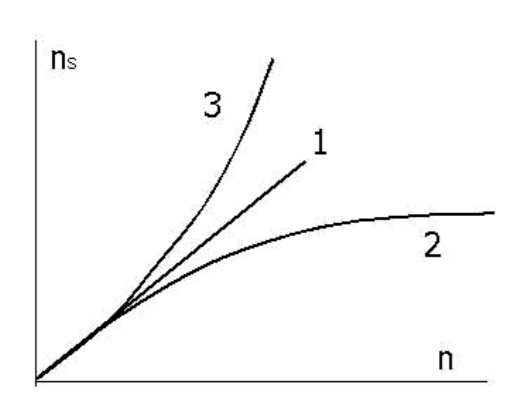
\includegraphics[width=10cm,height=6cm]{1}}
\caption{Изотермы сорбции: 1) Генри, 2) Ленгмюра, 3)  полислойной
адсорбции.}
\label{ris:image}
\end{figure}
Притяжение нейтральных молекул друг к
другу обусловлено силами Ван-дер-Ваальса, между полярными молекулами имеется
диполь-дипольное взаимодействие, ион-дипольное взаимодействие имеет место между
полярнай молекулой и нескомпенсированным зарядом поверхности, полярная молекула
может поляризовать нейтральную молекулу и взаимодействовать с наведенным диполем. \\
Наиболее прочная связь образуется в том случае, когда перераспределение электронов
между поверхностными и адсорбируемыми атомами приводит к образованию химической
связи. Это явление называется хемосорбцией, величина Q при хемосорбции имеет
порядок величины 100 кДж/моль. Связывание с поверхностью, при котором энергия
адсорбции не превышает нескольких десятков кДж/моль, принято относить к физической
адсорбции. Теплота адсорбции определяет время пребывания адсорбированной молекулы в
связанном состоянии на поверхности и играет ключевую роль в процессе
хроматографического разделения.
\subsection{ Время удерживания и высота эквивалентной теоретической тарелки ВЭТТ}
Обозначим длину колонки за L, а радиус -- за $\rho$. Время пребывания молекулы в колонке(\textit{время удержания}) $t_1$ складывается из времени движения в элюенте $t_0$ и времени пребывания в адсорбенте $t_s$: $t_1 = t_0 + t_s$. Введём коэффициент $\mu = t_s/t_0$, таким образом, $t_1 = t_0(1 + \mu)$. Количество молекул в  подвижной фазе составляет$ M = 2\pi\rho Ln_s$, в неподвижной -- $G = \pi\rho^2Ln$. Вспоминаем, что $W_a = W_d$ и получаем: 
\begin{equation}
\frac{G}{t_0} = \frac{M}{t_s} = \frac{M}{t_1 - t_0},
\end{equation}
выражаем отсюда $t_1$:
\begin{equation}
t_1 = t_0(1 + \frac{M}{G}) = t_0(1 + \frac{2n_s}{\rho n}).
\end{equation}
Заметим, что $\chi = \frac{2\mu}{\rho}$. Таким образом, из времени удержания легко выражается теплота адсорбции.
Эффективное разделение веществ происходит при достаточно сильной адсорбции, т.е. при $\mu \gg 1$. Поэтому, $t_1 \sim \mu t_0 \sim \chi$.  Обозначим скорость элюента за $\nu_0$, тогда $t_0 = \frac{L}{\nu_0}$.\\
\textbf{Высота эквивалентная теоретической тарелки}(ВЭТТ) равна длине участка колонки, на котором успевает установиться сорбционное равновесие. Предполагается, что время установления равновесия $\tau$ определяется временем диффузии молекул из объема к поверхности, $\tau \sim \frac{\rho^2}{D}$, где D -- коэффициент диффузии в элюенте. ВЭТТ определятеся как $H = \nu_0\tau$, а количество тарелок в колонке $r = \frac{L}{H} \approx \frac{LD}{\nu_0\rho^2}$.
\begin{figure}[!h]
\center{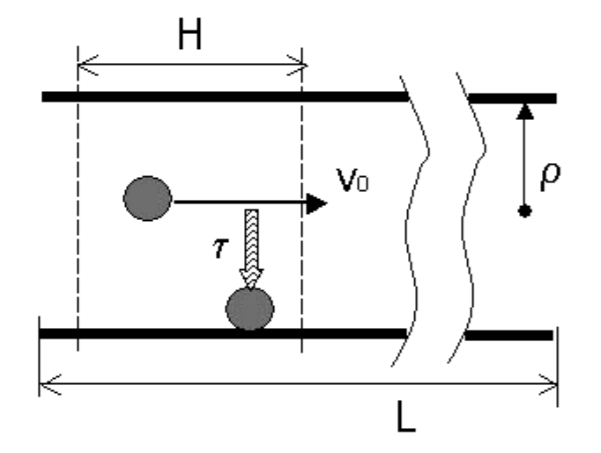
\includegraphics[width=6cm,height=4cm]{2}}
\caption{Иллюстрация понятия ВЭТТ.}
\label{ris:image}
\end{figure}
\subsection{Формирование хроматографического пика}
Процесс формирования
хроматографического пика удобно рассматривать, разбив
длину колонки L на отрезки длины Н и предполагая, что напуск газа-носителя
происходит порциями, заполняющими отрезки колонки длиной Н.\\
Введем вероятность р нахождения молекулы в элюенте, тогда $p = \frac{t_0}{t_1} = \frac{t_0}{t_0 + t_s} = \frac{1}{1 + \mu}$. Тогда вероятность нахождения молекулы на сорбенте равна $(1 - p) = \frac{\mu}{1 + \mu}$. Ввод каждой новой порции переводит все молекулы подвижной фазы на тарелку вперёд. Многократный напуск газа-носителя для сорбируемых молекул можно рассматривать как серию бинарных испытаний, таким образом вероятность нахождения молекулы в элюенте описывается биномиальным распределением. Биномиальное распределение позволяет рассчитать
вероятность Pn(r) того, что в серии из n испытаний «желаемое» событие произойдет r раз,
если вероятность его в единичном испытании равна р. 
\begin{equation}
P_n(r) = C_n^rp^n(1 - p)^{n-r},      C^r_n = \frac{n!}{r!(n - r)!}.
\end{equation}

	Молекула регистрируется детектором после прохождения ею r тарелок. Для типичных условий хроматографирования характерны следующие соотношения: $p \ll 1$(т.е. $\mu \gg 1$) и $n \gg r \gg 1$. Дискретное биномиальное распределение переходит в непрерывное распрпделение Гаусса при $n \rightarrow \infty$ и p = const. В этих условиях распределение принимает вид:
\begin{equation}
P_n(r) = \frac{1}{\sqrt{2\pi r}}exp\left[-\frac{(pn - r)^2}{2r}\right].
\end{equation}

	Функция (10) имеет колоколообразный вид с максимумом при $n_{max} =  \frac{r}{p}$. В качестве ширины пика $\Delta n$берут расстояние между точками, в которых значение функции уменьшается в $\sqrt{e}$ раз: $\Delta n = \frac{2\sqrt{r}}{p}$. В реальном эксперименте мы измеряем время удержания, поэтому необходимо сделать замену координаты $n \rightarrow t$. Легко понять, что t = n$\cdot\frac{t_0}{r}$. Тогда и $t_{max} = \frac{r}{p}\cdot\frac{t_0}{r} = t_0(1 + \mu) = t_1$. Соответственно, ширина пика $\Delta t = \frac{t_0}{r}\cdot\frac{2\sqrt{r}}{p} = \frac{2}{\sqrt{r}}\cdot t_1$. Таким образом, с увеличением числа тарелок пик сужается.\\
Условие, при выполнении которого два близких хроматографических пика окажутся разрешенными:
\begin{equation}
\frac{\mu_1 - \mu_2 }{\mu_1 + \mu_2} \geq \frac{1}{\sqrt{r}}
\end{equation}
Коэффициент $\mu$ непосредственно связан с константой Генри, которая зависит от теплоты
адсорбции Q молекулы на данной поверхности. По сути, формула определяет
минимальное различие в величинах Q, которое может быть зарегистрировано
хроматографическим методом при заданном числе тарелок r. \\
Разрешающая способность:
\begin{equation}
R=\frac{t}{\Delta t}=\frac{\sqrt{r}}{2}
\end{equation}
\subsection{Продольная диффузия и ширина пика}
Сужению пика способствует увеличение числа тарелок, но в то же время неограниченному сужению хроматографичекого пика препятствует процесс
диффузии вещества в направлении вдоль колонки (т.н. \textbf{продольная диффузия}).Формирование пика приводит к неоднородному распределению концентрации молекул,
что служит движущей силой продольной диффузии, результатом которой является
диффузионное уширение пика.\\
Оценим ширину хроматографического пика
$\Delta t_{dif}$, определяемую продольной диффузией. \\
Если в
начальный момент времени концентрация вещества в точке $x = 0$ составляла $C_0$, то в
момент времени t распределение концентрации С(х) будет иметь гауссову форму (решая дифференциальное уравнение): 
\begin{equation}
C(x,t) = C_0exp\left[-\frac{x^2}{4D^*t}\right],
\end{equation}
где $D^*$ -- эффективный коэффициент диффузии. Принимая за $D_s$ коэффициент диффузии в сорбенте, учитывая, что $Ds \ll D, \mu \gg 1$, получаем: $D^* = pD + (1 - p)D_s \approx pD = \frac{D}{1 + \mu} \approx \frac{D}{\mu}$. Тогда ширина пика $\Delta x_{dif} = 2\sqrt{2D^*t_1} = 2\sqrt{\frac{2D}{\mu}\cdot t_0\mu} = 2\sqrt{2Dt_0}$, в свою очередь $\Delta t_{dif} = \frac{\Delta x_{dif}}{\nu_1} = \frac{2\mu}{\nu_0}\sqrt{2Dt_0}$, где $\nu_1 = \frac{\nu_0}{1 + \mu}$ - скорость распостранения пика. В реальном эксперименте вклад в ширину пика вносят и адсорбционное и диффузионное уширение. Разрешающая способность тогда:
\begin{equation}
R = \frac{t_{max}}{\Delta t + \Delta t_{dif}}.
\end{equation}

Таким образом,
\begin{equation}
\frac{1}{R} = \frac{\frac{2}{\sqrt{r}}t_1 + \frac{2\mu}{\nu_0}\sqrt{2Dt_0}}{t_1} = 2(\frac{1}{\sqrt{r}} + \sqrt{\frac{2D}{L\nu_0}}) = \frac{2}{\sqrt{L}}\cdot\left(\sqrt{\frac{\nu_0\rho^2}{D}} + \sqrt{\frac{2D}{\nu_0}}\right). 
\end{equation}

Так как $H \sim \frac{1}{r}, a R^2 \sim r$, то $H \sim \frac{1}{R^2}$. Отсюда получаем \textbf{уравнение Ван-Деемтера}:
\begin{equation}
H \sim \left(\sqrt{\frac{\nu_0\rho^2}{LD}} + \sqrt{\frac{2D}{L\nu_0}}\right)^2 = A\nu_0 + \frac{B}{\nu_0} + C
\end{equation}
Уравнение Ван-Деемтера отражает немонотонный характер зависимости
ВЭТТ от скорости потока газа-носителя. Наличие минимума функции H($v_0$) означает, что существует оптимальная скорость $v_0$, при которой в данной
хроматографической колонке достигается наибольшая разрешающая способность.
\begin{figure}[!h]
\center{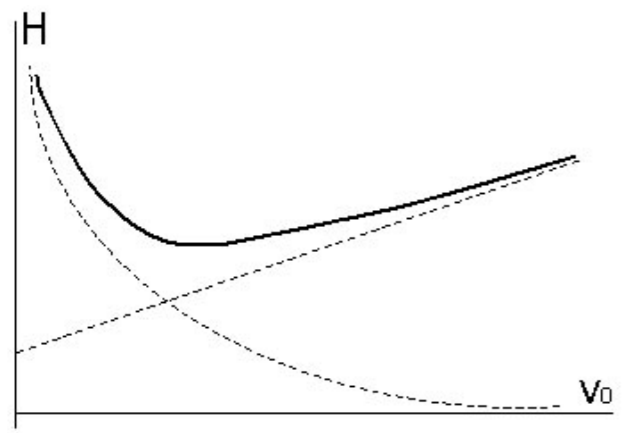
\includegraphics[width=6cm,height=4cm]{3}}
\caption{Зависимость ВЭТТ от скорости
потока газа носителя.}
\label{ris:image}
\end{figure}
\section{Методика}
\subsection{Устройство хроматографа}
Колонка непрерывно продувается потоком газа-носителя. Гелий из баллона через редуктор поступает в блок подготовки газов
(БПГ). Назначение БПГ – поддерживать стабильный заданный объемный расход газаносителя, который измеряется в мл/мин. Цифровой индикатор БПГ позволяет
контролировать соответствие заданного и текущего значения расхода. Погрешность
регулируемого БПГ расхода не превышает 1 мл/мин. Непостоянство скорости газаносителя приводит к погрешностям в определении времен удерживания и ширины пиков. Ввод анализируемой пробы в поток газа-носителя производится с помощью
дозирующего устройства (схема дозирующего устройства показана на рисунке 5). Важнейшее требование к дозирующему устройству –
постоянство объема водимой пробы.\\
\begin{figure}[!h]
\center{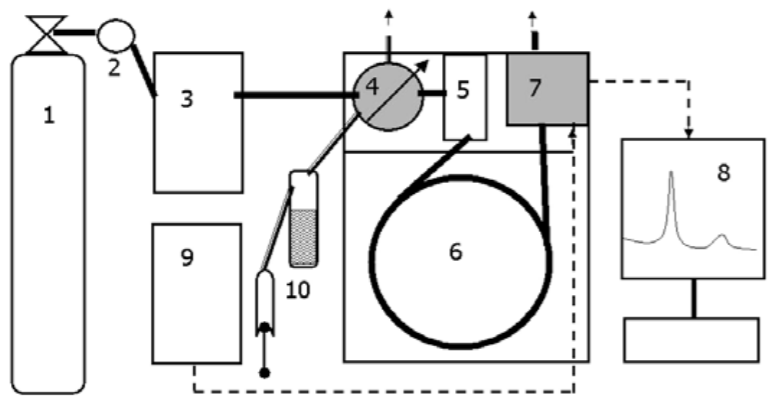
\includegraphics[width=8cm,height=4cm]{4}}
\caption{Блок-схема хроматографа: 1) баллон с газом-носителем, 2) редуктор, 3) блок
подготовки газов (БПГ), 4) кран-дозатор, 5) испаритель, 6) колонка в термостате, 7) детектор,
8) управляющий компьютер, 9) блок питания детектора (БПД), 10) система парофазного ввода
пробы (шприц, сосуд с парами).}
\label{ris:image}
\end{figure}
 \begin{figure}[!h]
\begin{center}
\begin{minipage}[h]{0.4\linewidth}
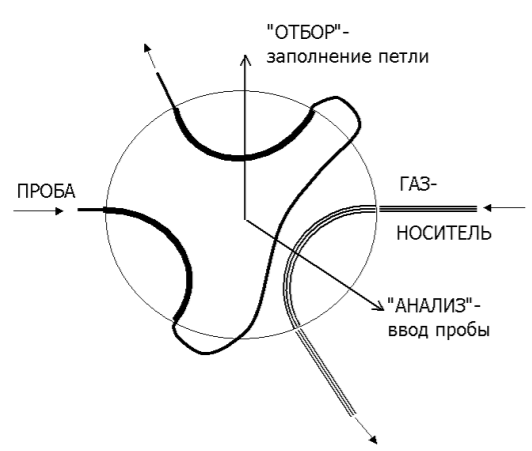
\includegraphics[width=1.0\linewidth]{5}
\caption{Схема поворотного крана-дозатора с
дозирующим объемом в виде трубки, установленной
на вращающейся втулке.} %% подпись к рисунку
\label{ris:experimoriginal} %% метка рисунка для ссылки на него
\end{minipage}
\hfill 
\begin{minipage}[h]{0.4\linewidth}
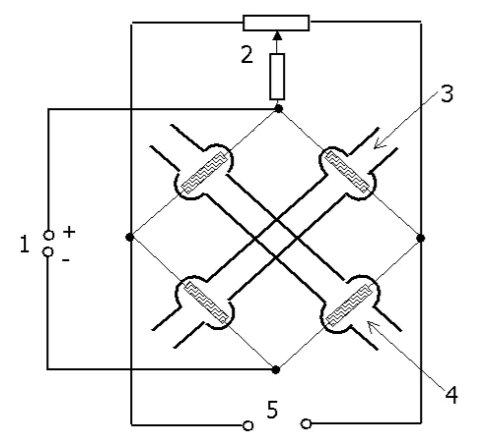
\includegraphics[width=1.0\linewidth]{6}
\caption{Пневмоэлектрическая схема ДТП.}
\label{ris:experimcoded}
\end{minipage}
\end{center}
\end{figure}
Перед попаданием в колонку проба
проходит через испаритель.
Назначение испарителя – перевод в
парообразную форму жидких образцов. Во избежание конденсации вещества в испарителе
его температуру поддерживают обычно на 30-50 К выше, чем температуру колонки. \\
Для регистрации анализируемых молекул в потоке газа-носителя на выходе из
колонки используется детектор по теплопроводности. Принцип действия ДТП основан на
сравнении теплопроводностей чистого газа-носителя и анализируемого вещества. 
\section{Экспериментальная часть}
\subsection{Определение теплоты адсорбции}
Чтобы определить какие пики соответствуют каким веществам, сначала снимаем хроматограмму пробы воздуха при температуре $180 ^0$C и расходе газа-носителя 30 мл/мин. Итого для смеси двух спиртов получаем 4 пика(см рис.7): первый - воздух, второй - вода, третий - этанол, четвертый - изопропанол.\\
\begin{figure}[!h]
\center{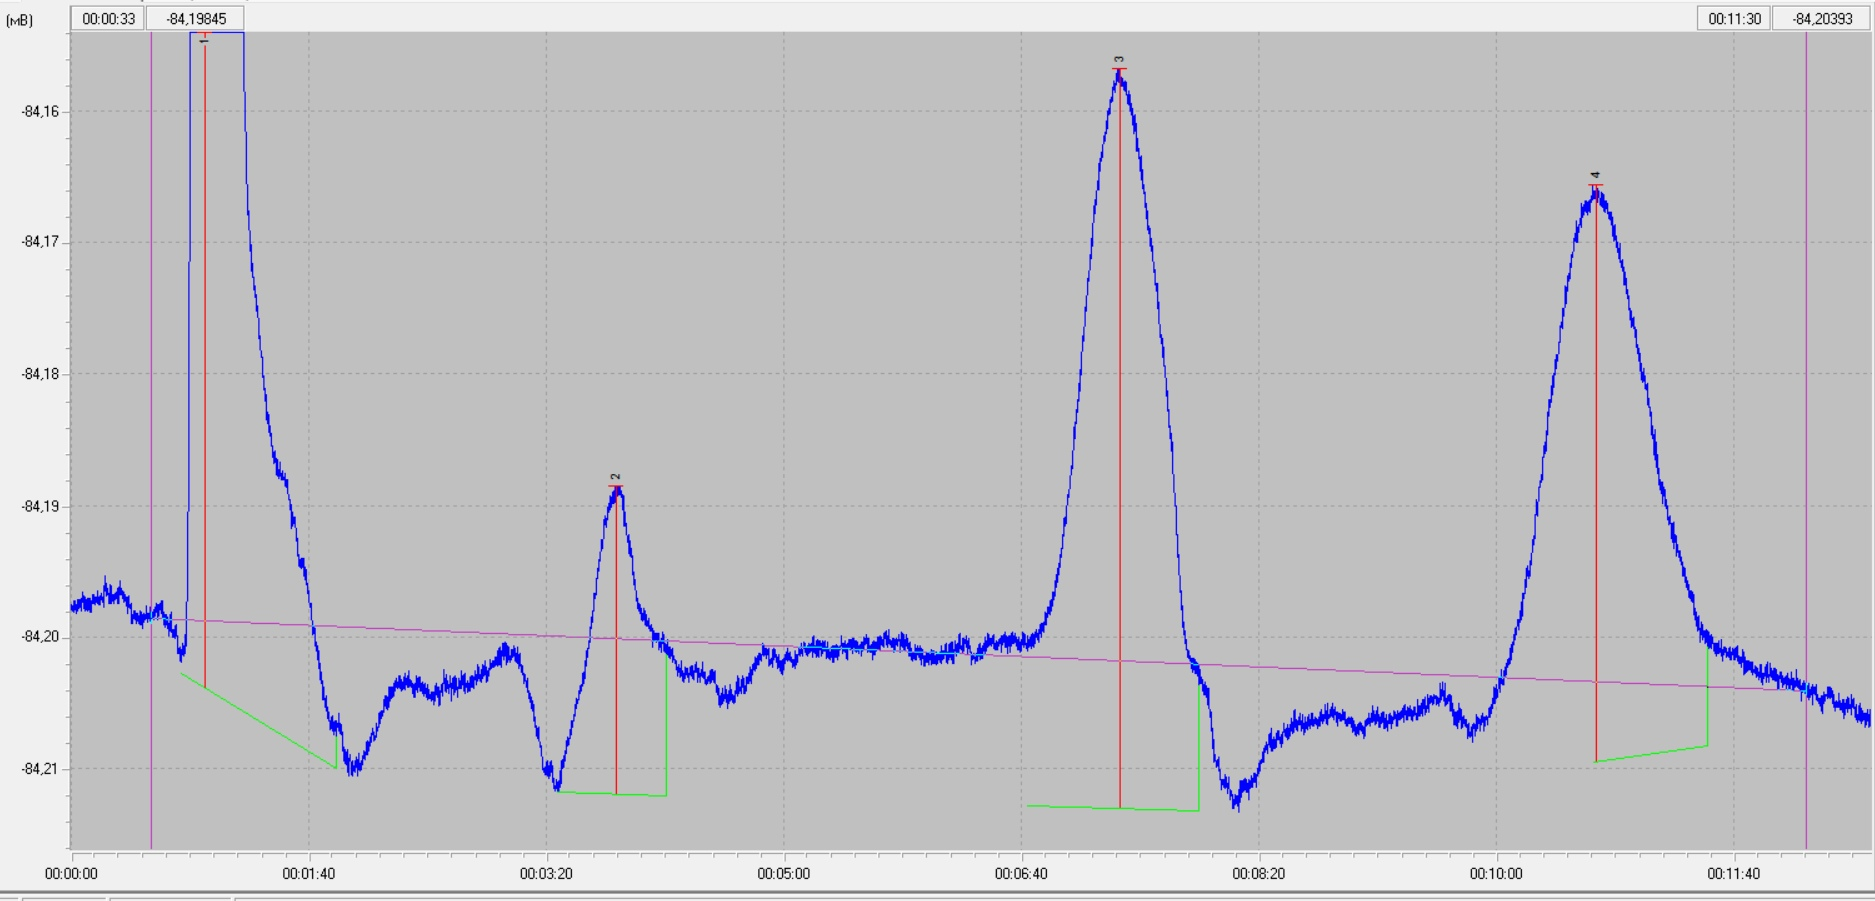
\includegraphics[width=16cm,height=7cm]{9}}
\caption{Хроматограмма смеси спиртов.}
\label{ris:image}
\end{figure}
Были получены хроматограммы смеси этанола и изопропанола при температурах в диапазоне $180-230^0$С с шагом в $10^0$С при постоянном расходе газа-носителя 30 мл/мин.
\begin{figure}[!h]
\center{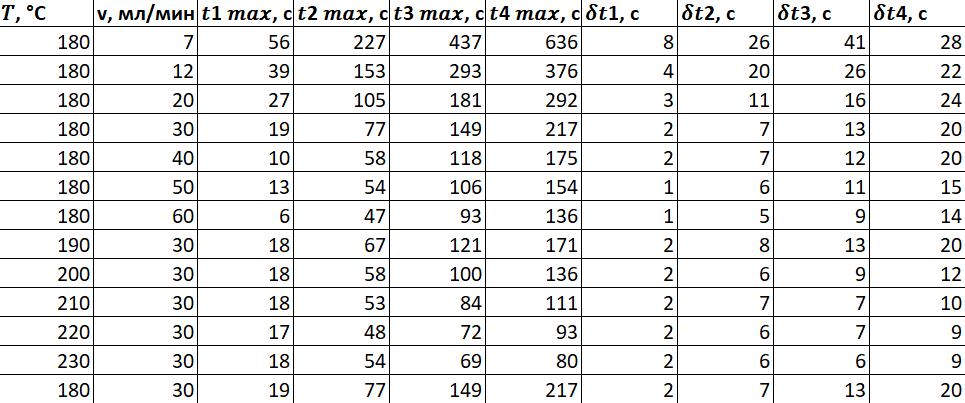
\includegraphics[width=14cm,height=6cm]{7}}
\caption{Таблица пиков хроматограмм при постоянном значении расхода газа-носителя и разных значениях температуры.}
\label{ris:image}
\end{figure}
Исходя из формул $\frac{n_s}{n}=\frac{v_T}{4} \cdot  \tau_0 \cdot e^{\frac{Q}{kT}}$ и $t_1=t_0 (1+ \frac{2n_s}{\rho n})$ имеем

\begin{equation}
 ln(\frac{t_1-t_0}{t_0} \frac{1}{\sqrt{T}}) = ln(\frac{1}{2\rho k_0} \sqrt{\frac{3R}{\mu}}) + \frac{Q}{kT}
\end{equation}

Учитывая это, можно найти теплоту адсорбции $Q$ по наклону наилучших прямых для графиков зависимости $ln(\frac{t_1-t_0}{t_0} \frac{1}{\sqrt{T}})$ от $\frac{1}{T}$.\\
\begin{figure}[!h]
\center{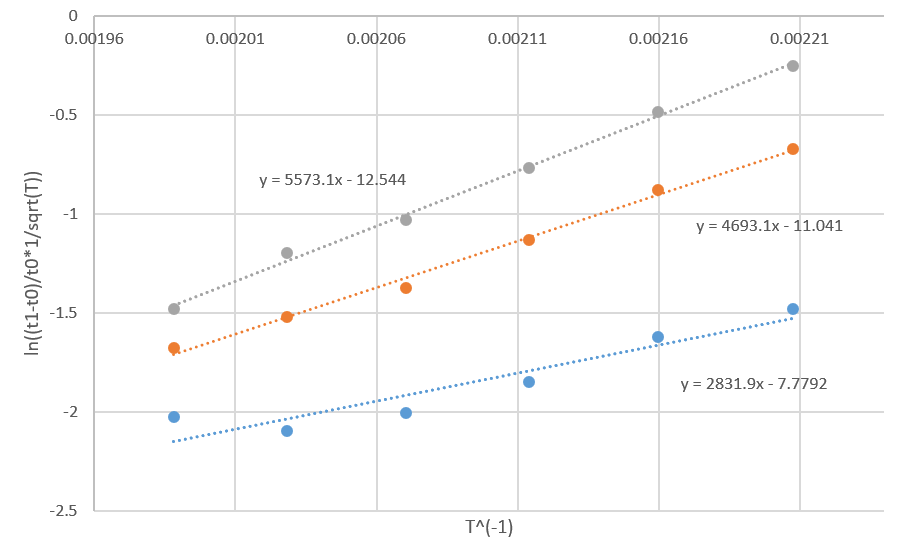
\includegraphics[width=14cm,height=8cm]{8}}
\caption{Таблица пиков хроматограмм при постоянном значении расхода газа-носителя и разных значениях температуры.}
\label{ris:image}
\end{figure}
\newpage
Рассчитаем теплоты адсорбции по формуле:
\begin{equation}
O=tan  \alpha kN_A = tan \alpha R
\end{equation}
$Q_{H_2O}$=($2.832 \pm 0.002$)кДж/моль\\
$Q_{Et}$=($4.693 \pm 0.05$)кДж/моль\\
$Q_{iPr}$=($5.573 \pm 0.2$)кДж/моль\\
Величины ошибок рассчитаны только с учетом отклонений зависимости от линейной.
Ширина пиков и другие источники ошибок не учитываются.

\subsection{Уравнение Ван-Деемтера}
Были получены хроматограммы ы при температуре $180^0$С при различном расходе
газа-носителя: 7, 12, 20, 30, 40, 50, 60 мл/мин (см рис.8).\\
Пользуясь определениями $R=\frac{t_max}{\delta t}$ и $H =\frac{L}{r}$, а также формулой $R=\frac{\sqrt{r}}{2}$ найдем разрешающую способность колонки по всем веществам при различных скоростях расхода.

\begin{figure}[!h]
\center{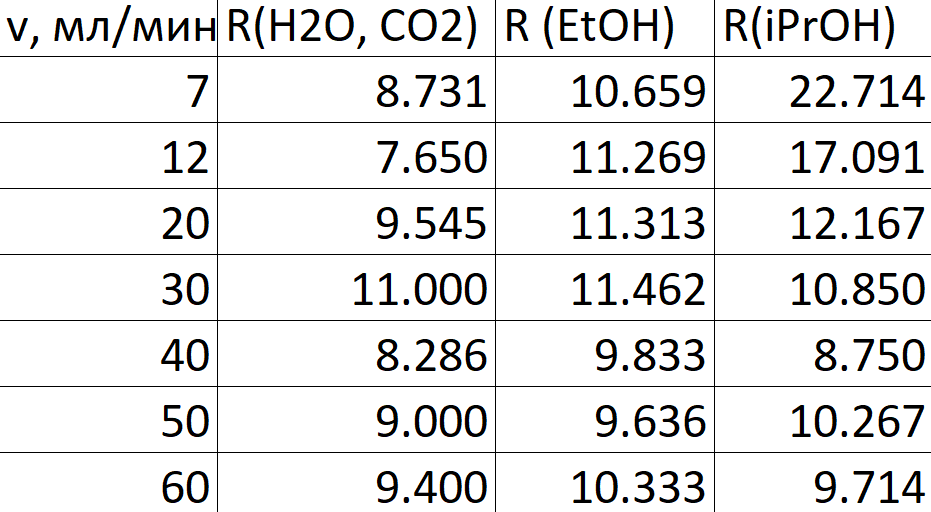
\includegraphics[width=6cm,height=4cm]{10}}
\caption{Разрешающая способность колонки для всех веществ при различных расходах.}
\label{ris:image}
\end{figure}
\begin{figure}[!h]
\center{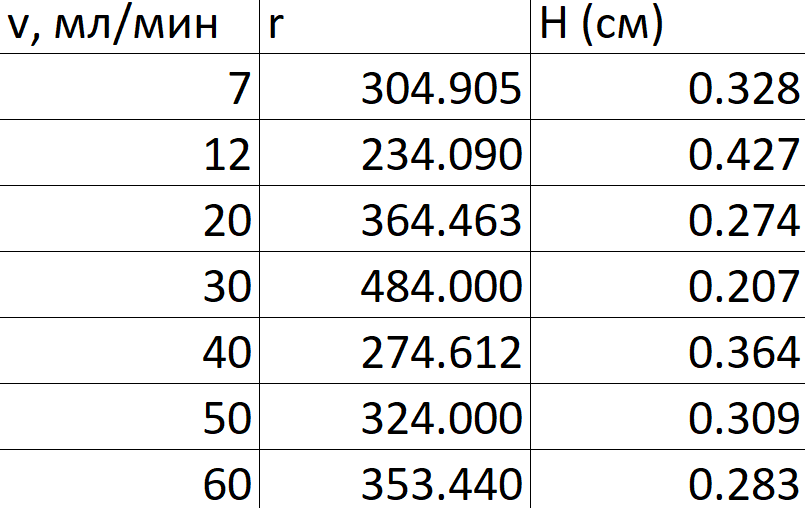
\includegraphics[width=6cm,height=4cm]{11}}
\caption{ВЭТТ и количество тарелок при разных значениях расхода газа-носителя.}
\label{ris:image}
\end{figure}
Найдем для каждого значения величины расхода количество тарело и ВЭТТ, используя
наименьшее значение разрешающей способности.
Построим график зависимости тарелок от расхода, и по нему определим оптимальную
величину расхода газа (см рис.12).
Уравнение Ван-Деемтера качественно подтвердилось. Из графика видна оптимальный
расход газа-носителя, который составляет 30 мл/мин. Отклонения при большем расходе
связаны с дрейфом и неточным определением ширины пика
\begin{figure}[!h]
\center{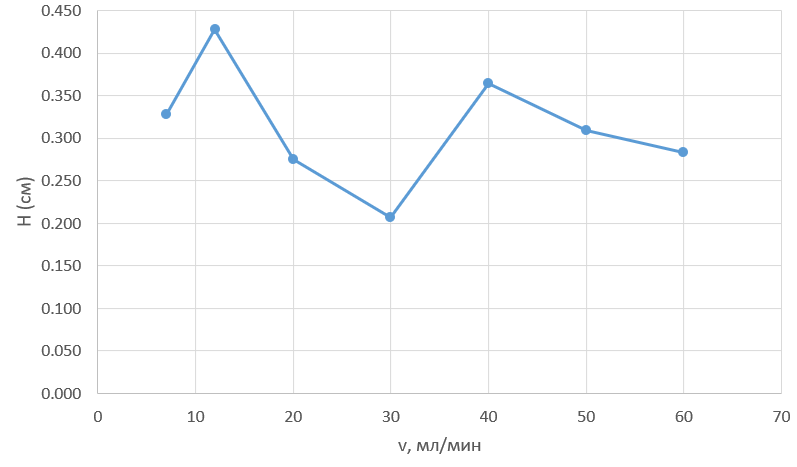
\includegraphics[width=12cm,height=8cm]{12}}
\caption{Зависимость ВЭТТ от расхода газа.}
\label{ris:image}
\end{figure}


\section{Обсуждение}
Из данных первой серии экспериментов найдены теплоты адсорбции для воды, этанола 
и изопропанола - $Q_{H_2O}$=($2.832 \pm 0.002$)кДж/моль,
$Q_{Et}$=($4.693 \pm 0.05$)кДж/моль,
$Q_{iPr}$=($5.573 \pm 0.2$)кДж/моль.\\ 
Полученные значения соответствуют энергиям физической адсорбции, что соответствует 
действительности - из структур порапака и веществ в эксперименте видно, что химической 
связи при сорбции образовываться не должно. 
Зависимости ВЭТТ от расхода газа-носителя имеет четкий минимум - $v_{opt}$ = 30 мл/мин.\\ 
По формам хроматографических пиков видно, что изотермы адсорбции воды, изопро- 
панола и этанола должны быть немного выпуклыми вверх, причем должны мало отли- 
чаться от прямых - предположение о применимости модели Генри оказалось верно. 
\section{Вывод}
Полученные хроматограммы показывают, что используемая в расчетах теория приме- 
нима в условиях эксперимента. Качественно выполняется закон Ван-Деемтера - зависимость ВЭТТ от расхода носителя имеет четкий минимум. 
Из зависимости положений пиков хроматограмм были вычислены теплоты адсорбции 
воды, этанола и изопропанола, соответствующие энергиям физической сорбции.
\section{Список литературы}
1. Адсорбционная
газовая
хроматография, описание лабораторной работы, ФБМФ 2009


\end{flushleft}
\end{document}